\documentclass[12pt]{article}
\usepackage[utf8]{inputenc}
\usepackage[T1]{fontenc}
\usepackage[spanish,es-lcroman]{babel}
\usepackage{amsmath}
\usepackage{amsthm}
\usepackage{physics}
\usepackage{tikz}
\usepackage{float}
\usepackage{cancel}
\usepackage[autostyle,spanish=mexican]{csquotes}
\usepackage[per-mode=symbol]{siunitx}
\usepackage{gensymb}
\usepackage{multicol}
\usepackage{enumitem}
\usepackage{stackengine}
\usepackage{stix}
\usepackage[left=2.00cm, right=2.00cm, top=2.00cm, 
     bottom=2.00cm]{geometry}

\usepackage{Estilos/ColoresLatex}
\usepackage{makecell}
\usepackage{wrapfig}
% \usepackage{titlesec}
\usetikzlibrary{angles,quotes}
\newcommand{\sectionbreak}{\clearpage}

\newcommand{\textocolor}[2]{\textbf{\textcolor{#1}{#2}}}
%\renewcommand{\questionlabel}{\thequestion)}

\newcommand{\Cancel}[2][black]{{\color{#1}\cancel{\color{black}#2}}}

\newcommand\deci[1]{%
    \kern-.4ex\stackunder[0.4pt]{$#1$}{$\color{blue}\acwunderarcarrow$}
}

\newcommand\decposl[1]{%    <--- Decimal position to left
    \kern-.4ex\stackunder[0.4pt]{$#1$}{%
      \reflectbox{$\color{red}\kern-.6ex\acwunderarcarrow$}
      }
}

\decimalpoint
\sisetup{bracket-numbers = false}

\title{\vspace*{-2cm} Piezoelectricidad}
\author{M. en C. Ramón Gustavo Contreras Mayén \\ {\fontsize{14}{14}\selectfont Universidad del Valle de México. Campus San Rafael}}
% \institute{Universidad del Valle de México. Campus San Rafael.}
\date{}

\begin{document}
\maketitle

\section{Piezoelectricidad.}

\subsection{Tipos de materiales.}

Para el tema de piezoelectricidad necesitamos comprender las diferencias entre algunos tipos de materiales.

A continuación se revisarán en qué consisten los:
\begin{enumerate}
\item Cristales.
\item Cerámicos.
\item Polímeros.
\end{enumerate}


\subsection{Cristales.}

Un material cristalino es una sustancia en la que sus átomos, iones o moléculas están dispuestos de manera ordenada y periódica en el espacio, formando una estructura tridimensional repetitiva llamada red cristalina.

Esta organización periódica se refleja en las propiedades físicas y químicas del material, lo que le confiere características únicas y distintivas.

\begin{figure}[H]
    \centering
    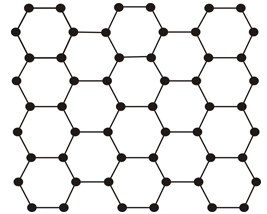
\includegraphics[scale=1]{Imagenes/Piezoelectricidad_01.png}
    \caption{Esquema en dos dimensiones de una red cristalina.}
\end{figure}
\begin{figure}[H]
    \centering
    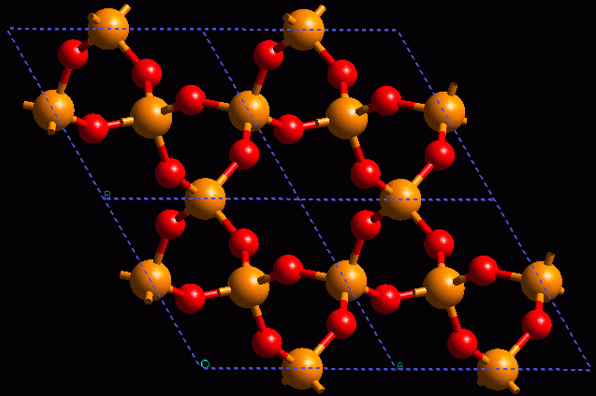
\includegraphics[scale=0.6]{Imagenes/Piezoelectricidad_02.png}
    \caption{Una red cristalina vista en 3D.}
\end{figure}


\subsection{Cerámicos.}

Los materiales cerámicos son una clase de materiales inorgánicos sólidos que están formados principalmente por compuestos metálicos y no metálicos unidos mediante enlaces iónicos o covalentes.
\begin{figure}[H]
    \centering
    
\includegraphics[scale=0.7]{Imagenes/Piezoelectricidad_03.jpg}
    \caption{Material base para un cerámico.}
\end{figure}

Estos materiales se caracterizan por su alta resistencia a la temperatura, dureza,  resistencia a la corrosión, y baja conductividad eléctrica y térmica.

Algunos ejemplos comunes de materiales cerámicos incluyen:
\begin{enumerate}
\item \textbf{Óxidos metálicos}:

Los óxidos metálicos, como el óxido de aluminio (alúmina), el óxido de silicio (sílice) y el óxido de titanio (titania), son algunos de los materiales cerámicos más comunes. Se utilizan en aplicaciones que requieren alta resistencia mecánica, resistencia al desgaste y resistencia a la corrosión, como abrasivos, aislantes eléctricos y revestimientos protectores.
\item \textbf{Compuestos no metálicos}:

Los compuestos no metálicos, como el carburo de silicio (carborundo) y el nitruro de silicio (silicon nitride), son otro tipo importante de material cerámico. Estos materiales tienen una alta resistencia a la temperatura y son utilizados en aplicaciones que requieren alta dureza, como herramientas de corte, rodamientos de alta temperatura y componentes electrónicos.
\item \textbf{Arcillas:}

Las arcillas son materiales cerámicos naturales compuestos principalmente por silicatos de aluminio hidratados. Se utilizan en la fabricación de ladrillos, tejas, cerámica de alfarería y porcelana debido a su capacidad para ser moldeadas y su bajo costo.
\item \textbf{Cementos:}

Los cementos son materiales cerámicos que se utilizan como aglomerantes en la construcción. El cemento Portland, que es una mezcla de cal, arcilla y otros minerales, es el tipo más común de cemento utilizado en la construcción de edificios, carreteras y otras estructuras.
\item \textbf{Vidrios:}

Aunque técnicamente no son cerámicos en el sentido estricto, los vidrios se consideran a menudo como parte del campo de los materiales cerámicos debido a sus similitudes en términos de estructura y propiedades. Los vidrios son materiales sólidos amorfos formados por enfriamiento rápido de líquidos fundidos. Se utilizan en una amplia variedad de aplicaciones, incluyendo envases, ventanas, fibra óptica y dispositivos electrónicos.
\end{enumerate}

Estos son solo algunos ejemplos de materiales cerámicos, nuevamente, mencionamos que estos materiales no necesariamente todos presentarán lo que conoceremos el efecto piezoeléctrico, la aportación de señalarlos nos servirá para ampliar nuestra conocimiento sobre los cerámicos.

\subsection{Polímeros.}

Los polímeros son macromoléculas formadas por la repetición de unidades simples llamadas monómeros.

Los polímeros se unen mediante enlaces covalentes para formar largas cadenas o redes, lo que confiere a los polímeros propiedades únicas y diversas.

A continuación se presentan algunos tipos de polímeros en general, lo que significa que no necesariamente presentaran el efecto piezoeléctrico que se mencionará más adelante, pero con fines de reconocer la gran utilidad de estos materiales, veremos que son tan comunes en nuestra vida diaria.

Tipos de polímeros:
\begin{enumerate}
\item \textbf{Polietileno (PE)}
El polietileno es uno de los plásticos más comunes y versátiles. Se utiliza en una amplia gama de aplicaciones, incluyendo envases de alimentos, bolsas de compras, botellas de plástico, aislantes eléctricos y tuberías.
\item \textbf{Poli(cloruro de vinilo) (PVC)}

El PVC es un plástico resistente y duradero que se utiliza en una variedad de aplicaciones, incluyendo tuberías, revestimientos para cables eléctricos, perfiles para ventanas y puertas, y productos de vinilo como suelos y revestimientos.
\item \textbf{Polipropileno (PP)}

El polipropileno es un plástico resistente al calor y a los productos químicos que se utiliza en una amplia variedad de aplicaciones, incluyendo envases de alimentos, componentes automotrices, textiles, y equipo médico.
\item \textbf{Poliestireno (PS)}

El poliestireno es un plástico transparente y rígido que se utiliza en aplicaciones como envases de alimentos, utensilios desechables, bandejas de semillas, y material de embalaje.
\item \textbf{Poliéster (PET)}

El poliéster es un polímero resistente al calor y a los productos químicos que se utiliza en aplicaciones como fibras textiles (por ejemplo, para hacer ropa y alfombras), envases de alimentos, botellas de plástico y películas de embalaje.
\item \textbf{Poliuretano (PU)}

El poliuretano es un polímero flexible y resistente que se utiliza en una variedad de aplicaciones, incluyendo espumas para colchones y muebles, recubrimientos impermeables, adhesivos y sellos.
\item \textbf{Polimetilmetacrilato (PMMA)}

El PMMA es un polímero transparente y resistente a los impactos que se utiliza en aplicaciones como ventanas de acrílico, paneles de visualización, lentes ópticas y prótesis médicas.
\end{enumerate}


\section{Piezoelectricidad.}
\subsection{Definición.}

La piezoelectricidad es un fenómeno físico en el cual ciertos materiales tienen la capacidad de generar una carga eléctrica, cuando se someten a una deformación mecánica o una presión externa, y viceversa.

A este efecto se conoce como efecto piezoeléctrico.

\vspace{0.3cm}
En la siguiente figura vemos como una presión, o una fuerza o un sonido actúa sobre el material piezoeléctrico, de tal manera que le genera una deformación mecánica, transformando esa energía mecánica en energía eléctrica, es decir, en un voltaje.
\begin{figure}[H]
    \centering
    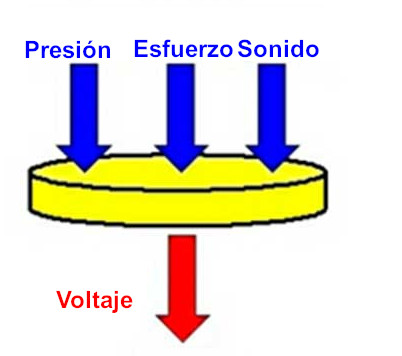
\includegraphics[scale=0.5]{Imagenes/Piezoelectricidad_04b.jpg}
    \caption{Transformación de energía mecánica a energía eléctrica.}
\end{figure}

Como se ha mencionado, un material piezoeléctrico también puede recibir energía eléctrica (voltaje) y en respuesta se transforma en energía eléctrica: ya sea vibración, fuerza, desplazamiento o sonido, que es lo que se muestra en la siguiente figura.
\begin{figure}[H]
    \centering
    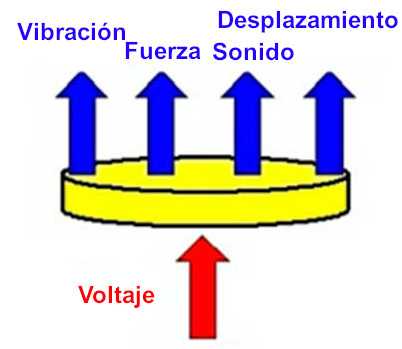
\includegraphics[scale=0.5]{Imagenes/Piezoelectricidad_04c.jpg}
    \caption{Transformación de energía eléctrica a energía mecánica.}
\end{figure}

Los materiales piezoeléctricos son aquellos que responden al efecto piezoeléctrico: ciertos materiales cristalinos, cerámicos y poliméricos.


\subsection{Materiales piezoeléctricos.}

Cristales.

\vspace{0.3cm}
Un cristal piezoeléctrico es un tipo de material cristalino que exhibe el efecto piezoeléctrico.

Este fenómeno se debe a la estructura asimétrica de los cristales piezoeléctricos, que permite la separación y el movimiento de las cargas eléctricas dentro del material en respuesta a una tensión mecánica.

Algunos de los cristales más comunes que exhiben propiedades piezoeléctricas son:
\begin{enumerate}
\item Cuarzo:

El cuarzo es uno de los cristales piezoeléctricos más utilizados. Tiene una alta estabilidad dimensional y una respuesta rápida a los cambios en el campo eléctrico.

Se utiliza en una amplia variedad de aplicaciones, incluyendo sensores, transductores ultrasónicos, relojes de cuarzo y dispositivos de filtrado.
\item Tourmalina:

La tourmalina es otro cristal que exhibe propiedades piezoeléctricas. Se utiliza en aplicaciones como sensores de presión, dispositivos de generación de energía y dispositivos de control de vibración.
\end{enumerate}

\section{Transformación de energía.}
\subsection{Mecánica a eléctrica.}

Cuando se aplica una fuerza mecánica o se produce una deformación en un material piezoeléctrico, los iones en la estructura cristalina del material se desplazan, generando una diferencia de potencial eléctrico a través del material. Esa diferencia de potencial eléctrico se captura utilizando electrodos colocados en la superficie del material piezoeléctrico.

Creando así una corriente eléctrica que puede ser utilizada para alimentar dispositivos electrónicos,  almacenada en una batería u obtener una señal eléctrica de algún dispositivo. En la siguiente imagen se representa la transformación de energía mecánica, con una onda sonora que incide sobre el material piezoeléctrico, se transforma a energía eléctrica y en conjunto con la electrónica, la señal eléctrica se conduce a otro elemento, por ejemplo: el uso de un micrófono.
\begin{figure}[H]
    \centering
    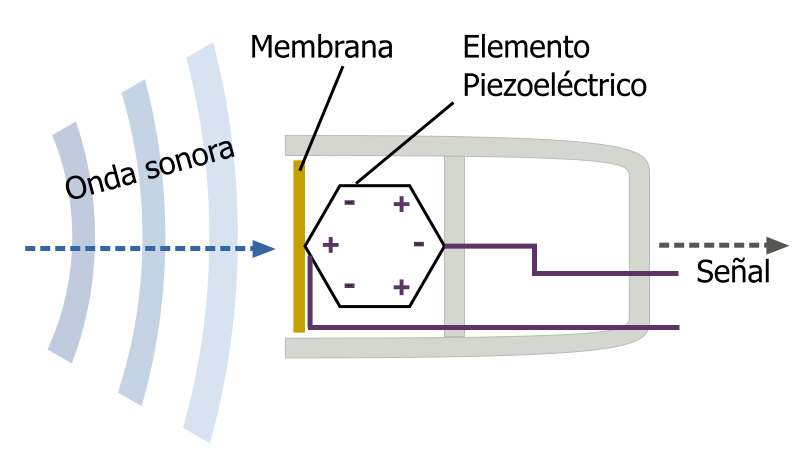
\includegraphics[scale=0.5]{Imagenes/Piezoelectricidad_05.png}
    \caption{Esquema de la transformación de energía mecánica a través del material piezoeléctrico, a energía eléctrica.}
\end{figure}

\subsection{Eléctrica a mecánica.}

Cuando se aplica un campo eléctrico externo a un material piezoeléctrico, los dipolos eléctricos dentro del material se alinean, causando una deformación o cambio en la forma del material.

Este proceso se utiliza en actuadores piezoeléctricos, donde la aplicación de un voltaje eléctrico controlado permite ajustar o mover dispositivos mecánicos con gran precisión.

\section{Aplicaciones.}

Algunas aplicaciones de la transformación de energía piezoeléctrica incluyen las siguientes:

\begin{enumerate}
\item \textbf{Sensores y transductores:}

Utilizados en aplicaciones como sistemas de monitoreo de presión, acelerómetros y sensores de vibración.

\item \textbf{Generadores de energía autónomos:}

Para la recolección de energía ambiental, como la vibración o el movimiento, y la alimentación de dispositivos electrónicos de baja potencia.

\item \textbf{Actuadores piezoeléctricos:}

En dispositivos de precisión, tales como microposicionadores, sistemas de enfoque automático, y sistemas de cancelación de vibración en vehículos y estructuras.
\end{enumerate}

La transformación de energía piezoeléctrica es un proceso importante que aprovecha las propiedades piezoeléctricas de ciertos materiales para convertir entre energía mecánica y eléctrica. Esta tecnología es ampliamente utilizada en una variedad de aplicaciones que requieren precisión, eficiencia energética y respuesta rápida.






\end{document}